\documentclass[12pt]{report}
\usepackage{lipsum}% for dummy text
\usepackage{titlesec}
\usepackage[utf8]{inputenc}
\usepackage[T1]{fontenc}\usepackage{lmodern}\usepackage{graphicx}
\usepackage[figurename=Fig.,labelfont=bf,labelsep=period]{caption}
\usepackage{subcaption}
\usepackage{newtxtext,newtxmath}
\usepackage[colorlinks=true,citecolor=red,linkcolor=black]{hyperref}
\usepackage{bm}
\usepackage{soul}
\usepackage{tikz}
\usepackage{ulem}
\usepackage{color}
\usepackage{cancel}
\usepackage{dsfont}
\usepackage{framed}
\usepackage{amssymb}
\usepackage{caption}
\usepackage{wrapfig}
\usepackage{amsfonts}
\usepackage{enumitem}
\usepackage{fancyhdr}
\usepackage{graphics}
\usepackage{lastpage}
\titleclass{\part}{top} % make\usepackage[utf8]{inputenc}
\usepackage[T1]{fontenc}\usepackage{lmodern}\usepackage{graphicx}
\usepackage[figurename=Fig.,labelfont=bf,labelsep=period]{caption}
\usepackage{subcaption}
\usepackage{newtxtext,newtxmath}
\usepackage[colorlinks=true,citecolor=red,linkcolor=black]{hyperref}
\usepackage{bm}
\usepackage{soul}
\usepackage{tikz}
\usepackage{ulem}
\usepackage{color}
\usepackage{cancel}
\usepackage{dsfont}
\usepackage{framed}
\usepackage{amsmath}
\usepackage{amssymb}
\usepackage{caption}
\usepackage{wrapfig}
\usepackage{amsfonts}
\usepackage{enumitem}
\usepackage{fancyhdr}
\usepackage{graphics}
\usepackage{lastpage}
\usepackage{multirow}
\usepackage{setspace}
\usepackage{algorithm}
\usepackage{algpseudocode}
\usepackage[mathscr]{euscript}
\usepackage{textcomp}
\usepackage{setspace}
\usepackage{lineno}
\usepackage{graphicx}
\graphicspath{{images/}}
\usepackage{eucal}
\usepackage{biblatex}
\addbibresource{references.bib}
\usepackage[style=authoryear,sorting=ynt]{biblatex}
\makeatletter
\newcommand*\bigcdot{\mathpalette\bigcdot@{.5}}
\newcommand*\bigcdot@[2]{\mathbin{\vcenter{\hbox{\scalebox{#2}{$\m@th#1\bullet$}}}}}
\makeatother
\titleformat{\part}
[display]
{\centering\normalfont\Huge\bfseries}
{\titlerule[5pt]\vspace{3pt}\titlerule[2pt]\vspace{3pt}\MakeUppercase{\partname} \thepart}
{0pt}
{\titlerule[2pt]\vspace{1pc}\huge\MakeUppercase}
%
\titlespacing*{\part}{0pt}{0pt}{20pt}
%
\titleclass{\chapter}{straight} % make chapter like a section (no newpage)
\titleformat{\chapter}
[display]
{\centering\normalfont\Huge\bfseries}
{\titlerule[5pt]\vspace{3pt}\titlerule[2pt]\vspace{3pt}\MakeUppercase{\chaptertitlename} \thechapter}
{0pt}
{\titlerule[2pt]\vspace{6pt}\huge\MakeUppercase}

\titlespacing*{\chapter}{0pt}{0pt}{40pt}
\title{apprentissage automatique préservant la confidentialité basé sur le chiffrement  homomorphique}
\author{Serigne Saliou Gueye }
\maketitle{}
\begin{document}
\chapter*{R E M E R C I E M E N T S}
Acknowledgement goes here
\chapter*{Resumé}
\chapter*{Intoduction générale}
\chapter*{Abstract}
\tableofcontents

\part{Contexte et introduction}
\chapter{Notion Préliminaires de la cryptographie}
Avant de passer à la définition du chiffrement homomorphe, nous allons revenir sur quelques notions cryptographiques à savoir les différents systèmes cryptographique (systèmes à clés secrètes et à clés privés) et aussi parler de la sécurité prouvée en cryptographie. Pour des traitements beaucoup plus approfondis de ces concepts nous renvoyons le lecteur sur \cite{1}
\section{Introduction}

La cryptographie est une discipline des maths incluant des principes et méthodes permettant de garantir  les services de sécurité de l’information .Sa principale mission  est de garantir la sécurité des communications c'est-à-dire de permettre à des entités qui ne se font pas confiance en général de communiquer en toute sécurité en présence de potentiels adversaires (susceptibles entre autres d'accéder à des secrets en violant la confidentialité, d'intercepter et de modifier les informations échangées ou d'usurper des identités lors d'une communication).
\\
La cryptographie ne prend en charge que les 4 premiers sur les 5 services de sécurité fondamentaux que sont la Confidentialité, l'intégrité, l'authentification, la Non Répudiation et la Disponibilité.Elle est composée des systèmes à clé secrète et des systèmes à clés publiques.
\\
 Dans un système à clés secrètes les entités se partagent la même clé pour le chiffrement et le déchiffrement (on parle de cryptographie symétrique)

 \\
 Dans le cas du système à clé publique, on utilise deux clés dont l'une soit k’ est difficile à déduire de l'autre soit k (on parle aussi de cryptographie asymétrique). La clé k est appelée clé publique et est utilisée pour le chiffrement ou la vérification de signature selon le système ; la clé k’ est appelée clé privée et est utilisée pour le déchiffrement ou la signature selon le système.
 \\

 Les algorithmes de chifffrements et les protocoles cryptographique sont impliqués dans une variété d'applications critiques:
 : les banques en ligne, le vote électronique, la vente aux enchères électroniques... En tant que tels, leurs securités doivent donc être formellement vérifiées et prouvées
 \section{Sécurité inconditionelle}
 \subsection{Notion de sécurité parfaite}
 Un cryptosytéme est parfois définis par trois algorithmes :Algorithme de génération des clés ,de chiffrement et de déchiffrement ainsi qu’une specification d’un espace de message M avec \#M > 1
 \\
 L’algorithme de génération des clés que nous notons GEN est un algorithme probabiliste qui produit une clé k choisit  selon une certaine distribution. Nous désignons par  K l’espace des clés c’est à dire l’ensemble de toutes les clés possibles qui peuvent être sortis par GEN
 \\
 L’algorithme de chiffrement que nous allons noté par ENC prend en entré une clé \kappa $ \in $ K et un messsage m $ \in $ M produit un  chiffré c .Nous considérons que l’algorithme de chiffrement est probabiliste donc ENC(k,m)peut alors générer des chiffrés différents lorsque le même message est utilisé.On note c \mapsto ENC{_\kappa}\[ \left (m\right ) \].On note C l’ensemble de tous les chiffrés possibles
\\
L’algorithme de déchiffrement noté par DEC prend en entré une clé $  \kappa $ et un chiffré c et produit le message initial m.
Contrairement à ENC l’algorithme de déchiffrement est déterministe puisque DEC{_\kappa}\[ \left (c \right ) \] donne la même sortie à chaque exécution on notera donc m:=DEC{_\kappa}\[ \left (c \right ) \]  pour designer le caractére deterministe
\\

Il est évident que si l’attaquant détient la clé  alors il pourra déchiffrer tous les messages échangés par les entités. Alors qu’en est-il de ENC ? N’est-il pas mieux de garder tous les deux (l’algorithme et la clé) secret?
\\
Auguste Kerckhoffs  a soutenu le contraire à la fin du 19e siècle lors de l’élucidation de plusieurs principes de conception de chiffrements militaires. L'un des plus important d’entre eux, désormais simplement connu sous le nom de principe de Kerckhoff.
\subsection{principe de Kerckhoff}
La méthode de chiffrement ne doit pas être tenue secrète, et elle doit pouvoir tomber entre les mains de l'attaquant sans inconvénient.
\\
Pour pouvoir bien comprendre ce principe et voir l’importance de garder la clé secrète nous pouvons considérer l’exemple suivant
\\
Soit m un message $\in$  $\{ 0,1 \}^n$ . On definit notre algorithme de chiffrement (ENC) en faisant la somme directe entre m et $\kappa$ $\in$ K
c = m  $\oplus$ $\kappa$ .On peut voir dans cet algorithme de chiffrement que si $\kappa$ est fixé
alors  ce cryptosystéme ne sera pas sur  et l'attaquant obtenir le massage initial à partir du chiffré en faisant m = c  $\oplus$ $\kappa$.
\\
Par contre si $\kappa$ est choisit de façon uniformément aléatoire   dans l’espace des clés $\{ 0,1 \}^n$ et gardé secret   pour l’attaquant alors le résultat du chiffré sera uniformément distribué dans l’espace des chiffrés $\{ 0,1 \}^n$  et la sécurité  sera atteinte
\subsection{Principe de Shannon}
Un chiffré doit apporter de la confusion et de la diffusion, c’est-à-dire :\\

Confusion \\
Il n’y a pas de relation algébrique simple entre le clair et le chiffré. En particulier, connaître un certain nombre de couples clair-chiffré ne permet pas d’interpoler la fonction de chiffrement pour les autres messages.\\
Diffusion\\
La modification d’une lettre du clair doit modifier l’ensemble du chiffré. On ne peut pas casser le chiffre morceau par morceau.
\subsection{Théoréme du secret parfait }
Avant d’énoncer ce théoréme,nous allons considérer les deux exemples ci-dessous \\
\subsubsection{exemple 1}
Considérons l’exemple simple du chiffrement de césar suivant\\
Soit $\kappa$ $\in$  $\{0,…….25\}$ avec Pr$\left[ K= \kappa \right]$     la probabilité que la clé soit k $\left$  (on considère  que les clés sont équiprobable)$ \right)$  donc Pr$\left[ K= \kappa \right]$= $\frac{1}{26}$ .
Supposons que nous avons la distribution suivante sur M:Pr$\left[ M= a \right]$  = 0,7 et Pr$\left[ M=z \right]$ = 0,3.$\left$  (Pr$\left[ M= a \right]$ probabilité que le message soit a et Pr$\left[ M= z \right]$ probabilité que le message soit z  )$ \right)$.Ainsi on cherche alors la probabilité que le message chiffré soit B\\
On peut voir qu'il n'y a deux possibilités :soit M=a et K=1 ,soit m=z et k= 2 .Par indépendance de M et K nous avons  Pr$\left[ M= a  \wedge K=1 \right]$ =Pr$\left[ M= a \right]$*Pr$\left[ K= 1 \right]$,de même Pr$\left[ M= z  \wedge K=2 \right]$ =Pr$\left[ M= z \right]$*Pr$\left[ K= 2 \right]$.\\Par conséquent,\\
  Pr$\left[ C= B \right]$=  Pr$\left[ M= a  \wedge K=1 \right]$ + Pr$\left[ M= z  \wedge K=2 \right]$
  = 0,7 $\frac{1}{26}$+0,3 $\frac{1}{26}$= $\frac{1}{26}$ donc \\Pr$\left[ C= B \right]$=$\frac{1}{26}$\\
  Nous pouvons également calculer la probabilité conditionnelle par exemple calculer la probabilité que le chiffré B soit issu de a ,Pr$\left[ a \mid B \right]$.En utilisant le théoréme de Bayes nous obtenons :

   $Pr$\left[M= a \mid C=B \right]$= \dfrac{ Pr\left[C= B \mid M=a \right].Pr\left[ M= a \right] }{ Pr\left[ C= B \right]$ }
  \\
Notons  que  $Pr$\left[C= B \mid M=a \right]$  = $\frac{1}{26}$ , puisque si M = a alors la seule voie C = B
peut se produire si $ \kappa $  = 1 ce qui se produit avec une probabilité de  $\frac{1}{26}$ \\

Donc   $Pr$\left[M= a \mid C=B \right]$= \dfrac{ Pr\left[C= B \mid M=a \right].Pr\left[ M= a \right] }{ Pr\left[ C= B \right]$ }=$\frac{\frac{1}{26}.O,7}{\frac{1}{26}}$

$Pr$\left[M= a \mid C=B \right]$=  0,7\\
Conclusion\\ on a Pr$\left[ M= a \right]$ = $Pr$\left[M= a \mid C=B \right]$=0,7 .\\
Ce résultat montre que  la probabilité d’avoir une information claire sur le claire a ne varie pas même si on connait son chiffré
B
\subsubsection{exemple 2}
Considérez à nouveau le chiffre de décalage, mais avec la distribution suivante sur M:\\

Pr$\left[ M= kim \right]$=0,5,      Pr$\left[ M= ann \right]$=0,2,         Pr$\left[ M= boo \right]$=0,3\\
Calculons alors la probabilité pour que le chiffré C soit égale à DQQ.La seule façon dont ce  chiffré peut
se produire est si M = ann et K = 3, ou M = boo et K = 2, ce qui arrive avec la
probabilité 0,2 · $\frac{1}{26}$ + 0,3 · $\frac{1}{26}$ = $\frac{1}{52}$.\\
Nous pouvons également calculer la probabilité que le chifré DQQ soit isuu de ann.? Un calcul comme ci-dessus en utilisant le théorème de Bayes
donne $Pr$\left[M= ann \mid C=DQQ \right]$ = 0,4\\
conclusion \\
On a   Pr$\left[ M= ann \right]$ &\neq $Pr$\left[M= ann \mid C=DQQ \right]$ dans cette exemple nous avons vu avec cette distribution  que la probabilité d’avoir une information claire  ann varie si son  chiffré DQQ est connu
\subsubsection{Commentaire}
Nous pouvons maintenant definir la notion de secret parfait .On imagine un adversaire qui connaît la distribution de probabilité de M
c’est-à-dire que l'adversaire connaît la probabilité que différents messages soient envoyés.\\
L'adversaire connaît également le schéma de chiffrement utilisé. La seule chose
Inconnue de l'adversaire est la clé partagée par les parties. Un message est
choisi par l'une des parties et chiffré, et le texte chiffré résultant est transmis à l'autre partie. L'adversaire peut espionner la communication des parties, et ainsi observer ce texte chiffré. (Autrement dit, c'est un
Attaque de texte chiffré uniquement « ciphertext-only attack », où l'attaquant ne voit qu'un seul texte chiffré.)\\
Dans un  schéma parfaitement secret, l'observation de ce texte chiffré ne devrait avoir aucun effet sur la connaissance de l'adversaire concernant le message réel qui a été envoyé; autrement dit, la probabilité a posteriori qu'un message m $\in$ M ait été envoyé,conditionné par le texte chiffré qui a été observé, ne devrait pas être différente de
la probabilité a priori que m serait envoyé. Cela signifie que le texte chiffré ne révèle rien sur le message envoyé sous-jacent et que l’adversaire n’apprend absolument rien sur le texte en clair qui a été chiffré. Formellement
\subsubsection{Definition 1}
Un cryptosystéme (GEN,ENC,DEC) avec M l’espace de messages est parfaitement secret si pour toute distribution de probabilité sur M et $\forall$ m $\in$ M et c $\in$ C telque Pr[C=c]>0 on a ;
\begin{center}
  $Pr$\left[M= m \mid C=c \right]$=   $Pr$\left[M= m \right]$.
\end{center}\\
(L'exigence que Pr [C = c]> 0 est une condition nécessaire pour éviter le
Conditionnement sur un événement à probabilité nulle.)
\\
Nous pouvons voir que le chiffrement de césar n’est pas parfaitement secret

\subsubsection{Théorème du secret parfait, Shannon }
Soit (M,K,C, GEN,ENC,DEC) un cryptosytéme .On suppose que \#M =\#K =\#C <$\infty$ et que Pr[M=m]>0 $\forall$ m $\in$ M .
Alors ce cryptosytéme est à secert parfait Si seulement si

 $\bigcdot$ La distribution des clés suit une loi uniforme \\

 $\bigcdot$ pour tout clair m appartient à M\\
\begin{center}
  \[ \phi{_m} =
  \begin{cases}
  K$\longrightarrow$C\\
  $\kappa$$\longrightarrow$ENC{_\kappa}\[ \left (m\right ) \]
  \end{cases}
\]
\end{center}


est une bijection
\subsubsection{Démonstration}
On suppose avoir secret parfait. On montre d’abord la bijectivité, puis l’équiprobabilité.
Bijectivité\\
S’il existe m tel que \phi_m:k\mapsto $ENC{_\kappa}\[ \left (m\right ) \]  est non surjective, il existe c $\in$ C tel que $\forall$ \kappa $\in$ K, $ENC{_\kappa}\[ \left (m\right ) \]\neq c$. En particulier Pr$\left[C= c \mid M=m \right]$=0, d’où l’on tire Pr$\left[M=m  \mid C=c \right]$=0\neq\Pr$\left[M=m \right]$>0 impossible. Donc $ \phi_m$  est surjective, et par égalité des cardinaux bijective.
\\
Equiprobabilité\\
Soit c $\in$ C un chiffré fixé. Pour tout m $\in$ M, on note $\kappa$(m) l’unique clef telle que $ENC{_$ \kappa(m)$  }[m]=c (d’après la bijectivité). On a Pr$\left[M=m  \mid C=c \right]$ = Pr$\left[K=$\kappa$(m) ]\right]$

Puisque par hypothèse Pr$\left[M=m  \mid C=c \right]$=Pr$\left[M=m \right]$, on obtient Pr$\left[K=$\kappa$(m) ]\right]$=Pr$\left[C=c \right]$.Or le chiffrement m\mapsto $ENC{_\kappa}\[ \left (m\right ) \]  est injectif à clef fixé, donc bijectif. Donc pour toute clef $\kappa$, il existe m tel que $\kappa$=$\kappa$(m).

Ainsi, Pr$\left[K=$\kappa$ ]\right]$ = Pr$\left[K=$\kappa$(m) ]\right]$ = Pr$\left[C=c ]\right]$est constante, et vaut  $\frac{1}{\#K}$

Dans le sens réciproque, il suffit d’effectuer le calcul : par équiprobabilité des clefs
\section{définition de sécurité pour la cryptographie à clé privée}
Avant de parler de la sécurité, nous allons définir formellement ce que signifie être  sùr  pou un  système cryptographique .La sécurité d’un cryptosysteme est évaluée du fait qu’un adversaire efficace  peut ou non différencier ou distinguer le chiffré de deux textes clairs  dans une preuve par jeux donnée .
\subsubsection{Fonction négligeable }

  Une fonction F de $\mathbf{N} & \longrightarrow &\mathbf{R}$ est dite negligeable  si pout tout polynome P il existe n{_0} $\in$ N telque pour tout n> n{_0}$  on a:
  \begin{center}
    F(n)<$\frac{1}{ P\left(n\right) } $

  \end{center}
  Dans ce qui suit le terme on utilisera le terme  « securité eav» pour  désigner  la sécurité  du preuve par jeu en présence d’un espion comme noté dans la [référence]

  \subsection{sécurité EAV }
  \subsubsection{indistinguabilité}
  On considère une expérience noté PrivK^{eav}$  dans lequel un adversaire A émet deux messages m{_0},m{_1}$  et recoit le chiffré d’un de ces messages .La définition de l’indistinguabilité stipule qu’un schèma E est sûr  si aucun adversaire A  ne peut déterminer lequel des deux messages a été chiffre on dit alors que le cryptosysteme est indistinguable
  \subsubsection{Définition de l'expérience}
  L’expérience est définie pour un schéma de chiffrement à clé privée E = (GEN, ENC, DEC), un adversaire A, et une valeur n pour le paramètre de sécurité :\\
  1 ) L'adversaire A émet deux messages m{_0}, m{_1} $\in$ M
  \\
  \\
  2)Une clé $\kappa$ est générée à l’aide de l’algorithme GEN, inconnue de l’adversaire de plus un bit aléatoire b  $\in$
   $\{0,1\}$ est choisi pour sélectionner m{_0}, m{_1} $ . On calcule  c=$ENC{_\kappa}\[ \left (m{_b}\right ) \] et on donne le chiffré c à   A comme challenge
   \\
   \\
   3)A émet alors un bit b ‘ dans le but d’avoir b’=b
   \\
   \\
   4 ) Le résultat de l’expérience est 1 si b’=b et 0 sinon .Dans le cas ou le résultat est 1  on dit que A a réussi et on note  PrivK^{eav}{_A,_E}$  =1\\
Ainsi formellement nous pouvons definir la « securité EAV » comme suit\\
\subsubsection{Définition 2}
Un schéma de chiffrement à clé privée E= (GEN, ENC, DEC) est indistinguable sous une attaque eav(attaque en présence d'espion) si pour tout algorithme probaliste ,il existe une fonction negligeable negl  telle que
\begin{center}
   Pr$\left[PrivK^{eav}{_A,_E}$(n) =1  ]\right]$ $\leq$ $\frac{1}{2}$  + negl(n)
\end{center}
Où la probabilité est prise aléatoirement  et l’expérience également (c'est-à-dire
le choix de la clé, du bit b ainsi que tout paramètre utilisé par ENC).
\subsection{Attaque par texte choisi (Choosen plaintext Attack CPA)}
Formellement, nous modélisons les attaques par texte choisi en donnant à l'adversaire A l'accès à un oracle de chiffrement, vu comme une boîte noire" qui chiffre les messages choisis par A à l'aide d'une clé k inconnue de lui.
Autrement dit, nous imaginons que A a accès à un "oracle" ENC{_$\kappa$}(-) ; lorsque A
interroge cet oracle en lui fournissant un message m comme entrée, l'oracle
renvoie un texte chiffré c ← ENC{_$\kappa$}(m) comme réponse. (Si ENC est randomisé, l'oracle
oracle utilise un nouvel aléa chaque fois qu'il répond à une requête). L'adversaire
peut interagir avec l'oracle de chiffrement de manière adaptative, autant de fois qu'il le souhaite.\\
\\
Considérons l'expérience suivante définie pour tout schéma de chiffrement E =
(GENC, ENC, DEC), l'adversaire A, et la valeur n pour le paramètre de sécurité :
\\
\\
1.) Une clé k est générée en utilisant GEN. L'adversaire A, qui ne connaît pas la clé, est autorisé à effectuer un nombre polynomial de requêtes à un oracle de chiffrement ENC{_$\kappa$}.
\\
\\
2.)A émet deux messages m{_0}, m{_1}$ $ $\in$ M
\\
\\
3.) On choisit un bit aléatoire b $\in$  $\{0,1\}$. On calcule c = ENC{_$\kappa$}(m{_b}$) et on donne  le chiffré c à A comme le challenge
\\
4.) A continue à avoir accès à l'oracle de chiffrement ENC{_$\kappa$}.
\\
\\
5.) A sort un bit b' dans le but d'avoir b'= b
\\
\\
6.) La sortie de l'expérience est 1 si b'= b et 0 sinon. Nous appelons le premier cas le succès de A et le désignons par
PrivK^{cpa}{_A,_E}$  =1\\.
\subsubsection{Définition 3}
Un schéma de chiffrement à clé privée E = (GEN, ENC, DEC) est sûr en cas d'attaque par texte plat choisi
(CPA) si, pour tous les adversaires probabilistes en temps polynomial A, il existe une fonction négligeable negl
telle que
\begin{center}
  Pr$\left[PrivK^{cpa}{_A,_E}$(n) =1  ]\right]$ $\leq$ $\frac{1}{2}$  + negl(n)

\end{center}
\subsubsection{proposition 1}
Un schéma de chiffrement E dont l’algorithme de chiffrement ENC  est déterministe ne peut pas être CPA-sûr
\subsubsection{Démonstration}
Considérons l'adversaire A suivant qui joue le jeu de sécurité CPA comme suit :\\
1.) Sélectionner  deux messages aléatoires distincts m{_0}, m{_1}$  $\in$ M.\\
2.) Utiliser l'oracle de chiffrement pour obtenir les chiffrés c{_0} = ENC{_$\kappa$}(m{_0}$) et c{_1} = ENC{_$\kappa$}(m{_1}$).\\
3.) Sortir les deux messages m{_1}, m{_1}$  $\in$ M\\
4.) A la réception du texte chiffré c, si c = c{_0}$ , sortir le bit 0, sinon sortir le bit 1.\\
Comme ENC est déterministe, le texte chiffré du challenge  c, étant un chiffrement de m{_0}$  ou m{_1}$ , sera égal à c{_0}$   ou c{_1} $ . Ainsi, A pourra réussir avec une probabilité non négligeable sur $\frac{1}{2}$ (en particulier,A réussira toujours). Ainsi, E ne peut pas être CPA-sûr
\subsection{Attaque à chiffré choisi (Choosen Cipher text Attack)(CCA)}
Qu’est-ce que cela signifie pour un schéma de chiffrement de résister contre les attaques à chiffre choisi ?
Comme d’habitude pour définir  une notion de sécurité appropriée, nous devons définir deux choses : la capacité supposé de l’attaquant et ce qui constitue une attaque réussie .Pour ce dernier nous suivrons l’approche adoptée dans les définitions précédentes .Nous allons   donc donner à l’attaquant un texte chiffré c comme challenge issu des messages m{_0}$  ou m{_1}$ (chacun choisi avec une probabilité égale )et on considère que le schéma est cassé si l’attaquant peut déterminer lequel des deux messages a été chiffre avec une probabilité significative meilleur que ½
\\
\\
L’attaque par chiffré choisi (CCA) permet à l’adversaire de disposer à la fois d’un oracle de chiffrement et de déchiffrement qu’il peut interroger à tout moment pendant le jeu.\\
D’autres textes distinguent les attaques par chiffré choisi non adaptative  et les attaques par chiffres choisis adaptative .Les premières également appelé  lunchtime permettent seulement à l’adversaire d’utiliser l’oracle de déchiffrement  avant de recevoir le challenge (le chiffré) .La seconde un modèle d’attaque beaucoup  plus puissant  permet à l’adversaire de continuer d’utiliser l’oracle de déchiffrement après avoir reçu le challenge ,mais évidemment il n’est pas autorisé à  interroger l’oracle de déchiffrement avec le challenge .
Dans ce mémoire nous faisons allusion à la seconde cas lorsque nous parlerons d’attaque CCA
Comme nous pouvons le voir la sécurité CCA est beaucoup plus forte que la sécurité CPA ou EAV et les implique tous les deux. Nous présenterons les définitions formelles ci-dessous\\
\\
Considérons l'expérience suivante définie pour tout schéma de chiffrement E =
(GENC, ENC, DEC), l'adversaire A, et la valeur n pour le paramètre de sécurité :\\
\\
1)Une clé est généré à l’aide de l’algorithme de génération  des clés GEN.L’adversaire A qui ne connait pas la clé ,peut effectuer un nombre polynomiale de requête à un oracle de chiffrement et de  déchiffrement \\
\\
2)A emet deux meaages m{_0}$  , m{_1}$
\\
\\
3)On choisit un bit aléatoire  b $\in$  $\{0,1\}$. On calcule c = ENC{_$\kappa$}(m{_b}$)et on donne c à A comme challenge \\
\\
4)A continué à avoir accès à l’oracle de chiffrement et de déchiffrement  mais avec la restriction que A ne peut pas exécuter l’oracle de déchiffrement sur le challenge c\\
\\
5)A produit un bit b’ dans le but d’avoir b’=b\\
\\
6)Le resultat de l’experience est  1 si b’=b et 0 sinon
Si b= b’ nous disons que A a réussi et nous le désignons par PrivK^{cca}{_A,_E}$  =1\\.
\subsubsection{Définition 3}
Un schéma de chiffrement à clé privée E = (KeyGen, Enc, Dec) est ,(CCA)  sûr si, pour tous les adversaires probabilistes en temps polynomial A, il existe une fonction négligeable negl telle que
\begin{center}
  Pr$\left[PrivK^{cca}{_A,_E}$(n) =1  ]\right]$ $\leq$ $\frac{1}{2}$  + negl(n)

\end{center}
\section{Cryptographie à clé publique }
\subsection{Fonction à sens unique }

Une fonction f : A $ \longrightarrow$ B est dite à sens unique s'il est facile
à calculer f(x) pour tout x ∈ A (complexité polynômiale)et est difficile (complexité
exponentielle) pour presque tout y $\in$ B, de trouver x tel que y = f(x).\\
\\
Une fonction est à sens unique avec trappe si l'on connaît un secret permettant de
l'inverser
\subsection{Fonction de hashage }
$\{ 0,1 \}^*$ ensemble des chaines de longueur quelconque, $\{ 0,1 \}^l$ ensemble des chaines longueur
fixe avec l$\neq$0.
\subsubsection{définition 3}

Une fonction H $\{ 0,1 \}^*$−→ $\{ 0,1 \}^l$ est dite fonction de hachage si :\\
1. Pour tout x, H(x) est facile à calculer, H(x) est appelé le hash ou l'empreinte de
x\\
2. Étant donné H(x), il est difficile de trouver y tel que y = H(x) (fonction à sens
unique) ;\\
3. Étant donné x, il est difficile de trouver x'tel que x $\neq$ x'et H(x) = H(x'), (collusions faibles) ;\\
4. Il est difficile de trouver x et x' (de son choix) x$\neq$= x'tel que H(x) = H(x'), (collusions
fortes) ;
\subsection{Modélisation du chiffrement à clés publique}
Un shéma de chiffrement à clé publique  de E=(GEN,ENC,DEC) avec un espace de clés $\mathcal{K}$= $\mathcal{K}${_k_s}$ $ $\times$ $\mathcal{K}${_k_p}$,un espace de message $\mathcal{M}$ et un espace  chiffré $\mathcal{C}$ est un 3-tuple d'algorithme efficace dans lequel :\\
GEN : $\lambda$ $\longrightarrow$$\mathcal{K}$ algorithme de génération des clés\\
ENC{_$\kappa$} : $\mathcal{M}$ $\longrightarrow$$\mathcal{C}$ est une fonction à sens unique (avec trappe qui est un inverse à gauche) appelée fonction de chiffrement et qui dépend d'un paramètre $\kappa$ appelé clé(publique)\\
DEC{_$\kappa$'} : $\mathcal{C}$ $\longrightarrow$$\mathcal{M}$ est la trappe  et est appelée fonction de déchiffrement (dépendant de la clé $\kappa$')  et on a DEC{_$\kappa$'}(ENC{_$\kappa$}(m)) = m
\\
\\
Il existe des définitions identiques  pour la sécurité EAV, CPA et CCA pour les systèmes de chiffrements à clé publique. Nous renvoyons  le lecteur à [référence] pour les détails.
\subsubsection{proposition 2}
Un cryptosystéme à clé publique est EAV-sùr si et seulement il est Cpa-sùr
\subsubsection{Démonstration}
Dans la version à clé publique du jeu de sécurité EAV, l'adversaire A a accès à la clé publique pk. Par conséquent, A peut calculer Enc{_p_k}$\left(m\right)$  lui-même pour tout message m, ce qui est équivalent à donner à A l'accès à un oracle de chiffrement. Par conséquent, pour les schémas de chiffrement à clé publique, la sécurité EAV est équivalente à la sécurité CPA.

\chapter{Le chiffrement homomorphe}
\section{Introduction}
A présent que nous avons vu les notions prélimnaires de la cryptographie,nous pouvons entammer  la theorie du chiffrement homomorphe.\\
Dans ce chapitre nous introduisons le concept du chiffrement homomorphe de maniére formelle mais aussi par analogie en utilisant  l'exemple  de la  bijouterie presenté dans \cite{3} .Ensuite nous allons parler de l'efficacité et de la sécurité du chiffrement homomorphe.\\
\section{ Concept du chiffrement homomorphe}
\subsection{Modélisation du chiffrement homomorphe}
\subsubsection{Définition}
Un cryptosytéme homomorphe $\varepsilon$  = (GEN,ENC,DEC,Evaluate ,F) avec $\mathcal{K}$ espace des clés ,$\mathcal{M}$ espace des  textes clairs $\mathcal{C}$ espace espace des textes  chiffrés  et $\lambda$ la paramétre de sécurité est un 5 uplet dont:\\
GEN : $\lambda$ $\longrightarrow$$\mathcal{K}$ est l' algorithme de génération des clés\\
ENC : $\mathcal{K}$ $\times$  $\mathcal{M}$ $\longrightarrow$$\mathcal{C}$ est l' algorithme de chiffrement\\
DEC : $\mathcal{K}$ $\times$  $\mathcal{C}$ $\longrightarrow$$\mathcal{M}$ l'algorithme de dechiffrement \\
Evaluate :  $\mathcal{F}$ $\times$ $\mathcal{C}^*$ $\longrightarrow$$\mathcal{C}$ est la fonction d'evaluation qui prend en entré une fonction autorisée f $\in$  $\mathcal{F}$ et l'évalue sur un ensemble de texte chiffré ($ $c{_1} $,$ $c{_2} $,......,$ $c{_n} $) pour produire un autre chiffré c .\\
\\

La definition ci ci-dessus stipule que si f represente une fonction de traitement alors on peut faire  du traitement (evaluer) sur les données sans en avoir accés .Cela peut sembler paradoxal ou voir impossible ,mais pour ce faire une  idéé de la solution  ,on peut considérer l'exemple suivant présenté dans l'étude de Gentry de 2010 \cite{3}.\\
Dans cette exemple Alice posséde une bijouterie.Elle prend des matiéres premieres dans son magasin (or, diamant ..)et les transforme en coliers et bagues. Alice doit s'occuper de la commande  des ses clients et elle est donc obligé à laisser à ses employeurs faire la transformation.Cependant Alice ne fait pas confiance à ses employeurs et elle craint qu'ils ne volent certaines matiéres premiéres à son insu.\\
La solution d'Alice à cette énigme est la suivante .Elle crée une boîte en laquelle elle seule a accés grace à une clé .La boite est accompagnée de gants qui permettent de manipuler  les objets qui s'y trouvent mais ne permettent pas de sortir quoi que soit de la boite .Ensuite Alice met les matiéres premieres dans la boîte et la ferme  avec sa clé pourque son contenu ne puisse pas etre retiré et demande à ses employés d'assembler les bijoux en utilisant les gants fournis par la boîte.\\
Ainsi Alice utilise sa clé pour ouvrir la boîte et récupérer les bijoux assemblés.\\
\\
Comme le note Gentry ,cette analogie présente en effet des insuffisances ,même  si les employeurs ne peuvent pas sortir les materiaux ,ils peuvent voir s'ils sont présent ou non et mieux ce que la boite contient,ce qui ne correspond pas aux exigeances de sécurité de la cryptographie.cependant l'exemple démontre suffisamment l'ideé prinicpale du chiffrement homomorphe.
\\
Une autre analogie, plus réaliste, est la suivante : supposons que la scolarité du département de LACGAA de l'UCAD  conserve des dossiers détaillés sur tous ses étudiants et leurs résultats.Ainsi la scolarité décide de  stocker tout ces données chiffrés évidement sur un service cloud .Ainsi les administrateurs de la scolarité veulent calculer à partir des données stockés sur le cloud la moyenne de chaque étudiants .Cependant ils ne veulent pas comprommettre les données personnelles des étudiants en donnant au service tier (le cloud) la clé secréte .\\
Dans ce cas si les administrateurs utilisent le chiffrement homomorphe où la moyennne sera une fonction autorisée( $\mu$ $ \in$ F),le service tie (cloud ) pourrra evaluer alors la moyenne des etudiants sur les donées chiffrés et le renvoyer à son tour aux administrateurs de la scolarité qui pouront alors utilisés leur clé secréte pour déchiffrer la moyenne chiffrée des étudiants .
\\
Notez que nous supposons que le service en cloud  suit un modèle honnête mais curieux, ce qui signifie qu'il exécutera les instructions correctement (c'est-à-dire qu'il calculera la fonction de chiffrement souhaitée au lieu d'une fonction malveillante de son choix), mais s'il en a l'occasion, il essaiera  d'obtenir des informations sur les données sous-jacentes chiffrés qu'il stocke.
\\
Cependant, il existe un cryptosytéme homomorphe trivial qui satisfait à notre définition du chiffrement homomorphe, où la fonction Evaluate ajoute simplement la description de la fonction aux chiffrés corresponds,et l'algorithme DEC se charge de l'evalution de la fonction on  a alors:
\begin{center}
  Evaluate(f, $c{_1}$, ..., $c{_n}$) = (f, $c{_1}$, ..., $c{_n}$) = c \\ L'algorithme DEC fait l'evaluation
  DEC(c) = f(DEC($c{_1}$), ..., DEC($c{_n}$))
\end{center}
\subsubsection{Definition 2}
Un schéma de chiffrement est dit compacte  si le temps d'exécution du déchiffrement du  chiffré évalué c (sortie de Evaluate) est égale au temps d'execution  du dechiffrement des chiffrés par lesquels il est crée  $c{_i}$ (entrée de Evaluate)
La taille c ne peut pas etre plus grande que la taiile des  $c{_i}$  et le temps de déchiffrement de c doit etre indépendant de la complexité de f, la fonction permise choisie.
\\
\\

\subsubsection{définition 3}
Un schéma de chiffrement homomorphe est dit à i-saut (i-hop homomorphe) s'il est possible d'appliquer le résultat de l'algorithme  d'évaluaion i fois de suite.
\\
\\
Une propriété intéressante que nous donne la compacité est que nous pouvons transformer un schéma de chiffrement homomorphe à clé privée en un schéma homomorphe à clé publique en particulier nous avons ce théorème suivant tiré de\cite{4}
\subsubsection{Théoréme }
Tout schéma de chiffrement à clé privée sécurisé à messages multiples qui est compact et homomorphe par rapport à l'addition modulo 2 peut être transformé en un schéma à clé publique sémantiquement sûr. \\En particulier, si le schéma à clé privée permet i + 1 évaluations de la fonction d'évaluation homomorphique((i+1)-hop homorphe)
alors le schéma à clé publique correspondant permet i évaluations de la fonction d'évaluation homomorphique(i-hop homomorphe)
\subsubsection{Démonstration}
Voir \cite{4} pour deux constructions explicites qui transforment de tels schémas de chiffrement à clé privée en schémas à clé publique.
\section{Sécurité des cryptosytémes homomorphe}
Par rapport à la sécurité des schémas de chiffrement  homorphes , il est important  de réfléchir su le modéle d'attaque du serveur tier (l'evaluateur) et voir  ce qu'il est capable de faire .Dans l'exemple précédent nous avons supposé que le modéle est honnête mais curieux ce qui signifie que la partie tierce (serveur ) suivra et exécutera les instructions correctementet essaiera d'en apprendre le plus possible sur les données chiffrés.\\
Notez qu'il y a d'autres modèles  beaucoup plus adverses que nous pouvons considérer pour le serveur (par exemple, il ne calcule pas toujours la fonction appropriée), mais ces obstacles présentés  peuvent être résolus en utilisant la délégation de calcul.cette derniére permet d'établir un protocole pour qu'un tiers calcule une fonction et prouve efficacement qu'il a correctement calculé la fonction .Nous allons pas dans ce mémoire traiter la délégation des chiffrements homorphe nous renvoyons le lecteur aux sources commme \cite{5}
\\
Une caractéristique des cryptosytémes homomorphes qui a des implications importantes pour la sécurité est la
malléabilité.
\subsection{La Malléabilité}
\subsubsection{Définition 3}
Un schéma de chiffrement E est malléable si, étant donné le texte chiffré d'un message, c = $ENC{_\kappa}\[ \left (m\right ) \],
il existe une fonction non constante f qui n'est pas la fonction d'identité, de sorte qu'un adversaire efficace A peut
calculer le texte chiffré d'un certain message lié  c' tel que $DEC{_\kappa}\[ \left (c'\right ) \] = f(m) avec une probabilité non négligeable.
\\
\\
Les cryptosytémes homomorphes sont malléables par définition  puisqu'ils permettent l'évaluation de diverses fonctions sur des chifffrés.Les cryptosytémes malléables sont intrinsèquement limités dans la sécurité qu'ils offrent.Les chercheurs ont montré que plus que le système est malléable, plus qu' il est facile à casser.Comme les cryptosystéme homorphes sont malléables , nous avons donc  la limitation suivante sur leur sécurité
\subsubsection{proposition 1}

Tout schéma de chiffrement malléable ne peut pas être sécurisé contre les attaques adaptatives par chifré choisi(CCA).
\subsubsection{Démonstration}
Soit E=(GEN,ENC,DEC,F,Evaluate) un cryptosystéme homorphe malléable où pour un certain message m{_0}$ ,et pout tout c $\in $
\begin{center}
  C{_m}$ =
  $\{ c$\in$ C | Pr$\left[ ENC{_\kappa}\[ \left (m{_0} \right ) =c\  \right]  avec $\kappa$ et ENC aléatoire\}$
\end{center}
Comme E est malléable alors le message f(m) a un chiffré de la forme g(c)  pour tout c $\in$ C{_m}$  où f, g peuvent être calculés en temps polynomial.Comme f est non constante, il existe un message m{_1}$  tel que f(m{_1}$ ) $\neq$ f(m{_0}$ ). Alors, on considère l'adversaire l'adversaire A suivant :\\
1.) Soumet m{_0}$  à l'oracle de chiffrement, et note c{_0}$  = ENC{$\kappa$}(m{_0}$ )\\
2.) Sort les messages f(m{_0}$ ) et f(m{_1}$ )\\
3.) A la réception du texte chiffré de défi c, A calcule g(c{_0}$ ). Si c = g(c{_0}$ ), alors la sortie b = 0. Sinon, tirer à pile ou face et sortir le résultat.
Nous pouvons voir qu'un tel adversaire obtiendrait un avantage non négligeable, et donc notre schéma de chiffrement
malléable E n'est pas sûr contre les attaques adaptatives par texte choisi.
\\\\
À partir de là, nous nous rendons compte que, bien qu'il existe des schémas de chiffrement, même à clé publique, qui sont sûrs contre les attaques par texte chiffré choisi adaptatif \cite{6}, il est impossible de construire un schéma de chiffrement homomorphe qui satisfasse à cette exigence de sécurité. Cela dit, bien que les schémas de chiffrement  homomorphes ne puissent pas
formellement répondre à l'exigence de la CCA, nous pouvons les augmenter avec des méthodes de délégation de calcul qui peuvent aider à garantir que le serveur ne modifie pas de manière malveillante les chiffrés qu'il renvoie, ce qui est le type d'attaque qui motive le désir d'une sécurité CCA \cite{5}. Il existe également de nombreuses d'autres normes de sécurité que les schémas de chiffrement homomorphes sont capables d'atteindre, comme la sécurité EAV et la sécurité CPA \cite{1}.\\
\\
 Les définitions de sécurité d'un chiffrement homomorphique sont les mêmes que celles d'un schéma de chiffrement simple. Pour un schéma de chiffrement régulier, imposant des conditions sur les opérations GEN, ENC, DEC, mais étant indépendantes de l'opération Evaluate.

\\
\\
\chapter{Notion Préliminaires de machine learning}
\section{Introduction}
Dans cette section, nous allons voir quelques algorithmes de machine learning qui seront combinés  ultérieurement avec les schémas de chiffrements homomorphes.Nous allons étudier les algorithmes d'apprentissage supervisé et non supervisé.\\
L'apprentissage supervisé consiste à déduire une fonction (modéle) à partir d'un ensemble de données  étiquetées.
Les deux types d'apprentissage supervisé sont la classification et la régression, le premier faisant référence au cas où les étiquettes forment un ensemble discret d'étiquettes de classe, et le second lorsque les étiquettes prennent des valeurs continues.Pour la classification , nous examinerons l' analyse discriminante linéaire ,  la classification naïve bayésienne et les arbres de décision.\\D'autre part, l'apprentissage non supervisé consiste à déduire la structure cachée des données non étiquetées.Pour le cas de l'apprentissage non supervisé ,nous allons voir l'nalyse en composantes principales,qui est également un outil important pour la réduction de la dimension\\
\section{Classification binaire}
La classification binaire est un  problème consistant à prendre un vecteur de caractéristiques \textbf{x} et à décider de laquelle des deux étiquettes (ou classes) il appartient. Par exemple  on peut prendre un vecteur de caractéristiques contenant la taille et le poids d'une personne et essayer de prédire  le sexe de la personne.Il existe de nombreux algorithmes qui traitent ce problème, notamment la régression logistique, les machines à vecteurs de support, etc.
Dans cette section, nous examinerons la discrimination linéaire de Fisher, qui est une technique permettant d'effectuer une classification binaire lorsque les caractéristiques sont des quantités continues.\\
L'analyse discriminante linéaire de Fisher aborde le problème de la classification en trouvant un vecteur \textbf{w} sur lequel
nous pouvons projeter les données sur un vecteur tel qu'il est plus facile de définir un point qui sépare les deux classes avec une grande marge. Pour ce faire, nous choisissons un vecteur w qui maximise le rapport entre les variances interclasse et intraclasse. Intuitivement, cela a du sens car nous voulons maximiser la séparation entre les différentes classes, tout en minimisant la séparation au sein de chaque classe. Une fois que nous avons ce vecteur \textbf{w}, nous pouvons classifier un point de données x en calculant $\textbf{w}^\intercal \mathbf{x}$ et en le comparant au seuil c correspondant à notre point de séparation.\\
\begin{figure}[h]
    \centeryy ning
    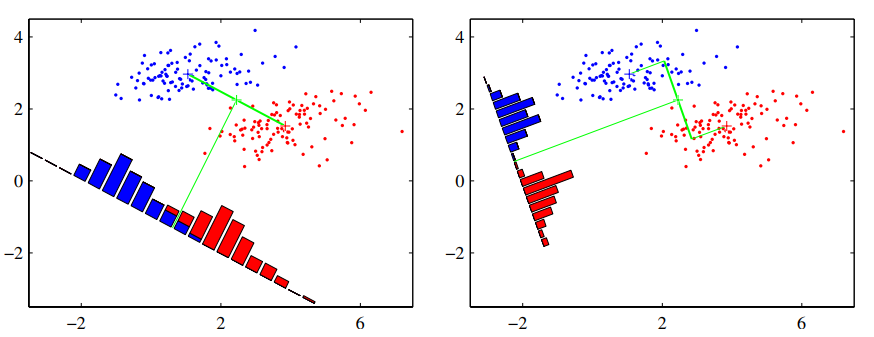
\includegraphics[width=1\textwidth]{1.PNG}

    \label{fig:figure 1}
\end{figure}\\

\\
De manière plus formelle,onsidérons un problème à deux classes dans lequel il y a N{_1}$  points de la classe C{_1}$  et N{_2}$  points de la classe C{_2}$ , de sorte que les vecteurs moyens des deux classes sont donnés par:
\begin{equation}
 u{_1}={\frac {1}{N{_1}}}\sum _{i=1}^{n}X_{i} ,  et    u{_2}={\frac {1}{N{_2}}}\sum _{i=1}^{n}X_{i}
\end{equation}
La mesure la plus simple de la séparation des classes, lorsqu'elle est projetée sur \mathbf{w}, est la
séparation des moyennes des classes projetées. Ceci suggère que nous pourrions choisir \mathbf{w} de manière à
maximiser
\begin{center}
  \begin{equation}
    u{_2}-u{_1}=\textbf{w}^\intercal (u{_2} -u{_1})

  \end{equation}
  \begin{equation}
    u{_k}=\textbf{w}^\intercal (u{_k})

  \end{equation}
\end{center}
La variance intra-classe des données transformées de la classe C{_k} $ est donc donnée par
\begin{center}
  \begin{equation}
    \sigma{_k}^2=\sum_{n \in C{_k}} (Y{_n}-u{_k})
  \end{equation}
\end{center}

où
\begin{equation}
  Y{_n}  = \textbf{w}^\intercal x{_n}
\end{equation}
 Nous pouvons définir la variance intra-classe totale pour l'ensemble des données comme étant simplement $\sigma{_1}^2$+$\sigma{_2}^2$. Le critère de Fisher est défini comme étant le rapport entre la variance interclasse et la variance interne à la classe et est donné par:\\
 \begin{equation}
   \begin{split}
     S  =\frac{\sigma^2{_(intra)}}{\sigma^2{_(extra)}}  \\  =\frac{(u{_2} -u{_1})^2}{\sigma{_1}^2+\sigma{_2}^2} \\  =\frac{(\textbf{w}^\intercal (u{_2} -u{_1}))^2}
     {
     (\sum_{i ,c{_i}=1}(\textbf{w}^\intercal(x{_i} -u{_1})))^2+ (\sum_{i ,c{_i}=2}(\textbf{w}^\intercal(x{_i} -u{_2})))^2
     } \\  =\frac{\textbf{w}^\intercal \mathbf{S{_B}}\mathbf{w}}{\textbf{w}^\intercal \mathbf{S}{_W}\mathbf{w}}
   \end{split}

 \end{equation}
 où $\mathbf{S{_B}}$ est la matrice de covariance entre les deux classes C{_1} $ et {C_2} $ avec \\
 \begin{equation}
   \mathbf{S{_B}}=(u{_2}-u{_1})(u{_2}-u{_1})^\intercal
 \end{equation}
 et $\mathbf{S{_W}}$ la matrice de covariance intra-classe avec
 \begin{equation}
   \mathbf{S}{_W} =\sum_{i ,c{_i}=1}(x{_i}-u{_1})(x{_i}-u{_1})^\intercal +  \sum_{i ,c{_i}=2}(x{_i}-u{_2})(x{_i}-u{_2})^\intercal
 \end{equation}
 En suivant la présentation de \cite{7}, nous pouvons deriver  par rapport à w pour obtenir
 \begin{equation}
   \frac{\partial{S}}{\partial{w}}=0 \Rightarrow (\textbf{w}^\intercal \mathbf{S{_B}}\mathbf{w})\mathbf{S}{_W}\mathbf{w}= (\textbf{w}^\intercal \mathbf{S}{_W}\mathbf{w})\mathbf{S{_B}}\mathbf{w}
 \end{equation}
 $\mathbf{S{_B}} \mathbf{w} $  est dans la même direction que  u{_2}$ -u{_1}$ et que $(\textbf{w}^\intercal \mathbf{S{_B}}\mathbf{w}) $ et  $(\textbf{w}^\intercal \mathbf{S}{_W}\mathbf{w})$ sont des constantes.
Puisque nous ne nous intéressons qu'à la direction et non au facteur  de $\mathbf{w}$, nous pouvons eliminer  les constantes et multiplier les deux côtés par  $\mathbf{S}{_W}^{-1}$ pour obtenir une solution optimale de w
\begin{center}
  $\mathbf{w}^{*}$ $\propto$  $\mathbf{S}{_W}^{-1}$(u{_2} $-u{_1} $)
\end{center}
Une fois que le $\mathbf{w }$ optimale calculé ,nous devons  trouver un seuil de classification c. D'habitude c est pris comme etant le  point médian entre les deux moyennes dans la direction donnée par $\mathbf{w}^{*}$.
\begin{equation}
     c = \frac{\textbf{w}^{*}^\intercal(u{_2}-u{_1})}{2}
\end{equation}
Ainsi, étant donné un point x, on calcule $\textbf{w}^{*}^\intercal$x et on classe  x selon que cette valeur est supérieure ou inférieure à c (seuil).

\section{Classification naïve bayésienne}
Un classificateur Naïve Bayes est une méthode pour classer des vecteurs  caractéristiques à valeur discrète. En particulier, étant donné un vecteur de données x $\in$  $\{1, ...K\}^n$, où K est le nombre de valeurs possibles pour chaque variable
 caractéristique et D est le nombre de variable caractéristiques. Cela nous permet d'écrire la densité conditionnelle de classe comme suit :
 \begin{equation}
    P(\mathbf{x} \mid C=c) =   \prod_{j=1}^D P(\mathbf{x}{_j} \mid C=c)
 \end{equation}
 Les classificateurs de Naïve Bayes sont qualifiés de ``naïves'' car ils supposent l'indépendance des variables ,ce qui est rarement le cas .Malgré cela , ils donnent parfois de bon résultat \cite{8}\\
 Comme son nom l'indique, les classificateurs Naïve Bayes constituent une autre façon d'aborder le problème de la classification.
Si nous avons K classes possibles, alors le modèle se compose de  classe de probabilité  à pirori $\{Pr(C = ci)\}_{i=1}^K$ (c'est-à-dire la probabilité à priori de la classe c{_i} $) et des densités conditionnelles de classe  $\{P(X = x | C = ci)\}_{i=1}^K$, c'est-à-dire la probabilité qu'un objet de la classe c{_i}$ possède un ensemble  de variables  caractéristiques  x.\\
À titre d'exemple , supposons que nous ayons une liste de maladies $\{m{_1}, ..., m{_n}\} $ et un vecteur de symptômes $(s{_1}, ..., s{_m})$  où s{_i}$=1 si la personne présente le symptôme i et 0 si elle ne le présente pas. Le modèle de Naïve Bayes spécifie P(s{_i} = 1 | m{_j}$) $\forall i,j $ (c'est-à-dire la probabilité qu'une personne présente le symptôme i étant donné qu'elle est atteinte de la maladie j) et P(m{_j} $ ) $\forall j $ (c'est-à-dire la probabilité qu'une personne soit atteinte de la maladie j). Ensuite, pour calculer la probabilité qu'une personne atteinte d'une maladie m{_k} $ présente un ensemble particulier de symptômes  $\(s'{_1}, ..., s'{_m}\)$, on calcule
\begin{center}
  P((s'{_1}, ..., s'{_m}) \mid m{_k} ) =   \prod_{j=1}^m P(s{_i}$  =s'{_i}$ \mid m{_k})

\end{center}
Avec ce modèle, la classification fonctionne alors en utilisant une règle de décision à posteriori maximale. Étant donné un point de données x, nous calculons la probabilité postérieure de son appartenance à chaque classe c{_i}$  et classons x dans la classe ayant la probabilité postérieure la plus élevée. Plus précisément, nous calculons.
\begin{equation}
\begin{split}

c^{*}=\DeclareMathOperator{\argmax}{arg\,max}_{i\in {1,....k}}P(C=c{_i} \mid X=x)=\DeclareMathOperator{\argmax}{arg\,max}_{i\in {1,....k}}\frac{P(X=x \mid C=c{_i})P(C=c{_i})}{P(X=x)}\\
=\DeclareMathOperator{\argmax}{arg\,max}_{i\in {1,....k}}P(X=x \mid C=c{_i}) P(C=c{_i})

\end{split}
\end{equation}
\\

Notez que dans la dernière étape, puisque P(X = x) est une constante pour toutes les classes le probléme se raméne alors à chercher des numeratuers  . Comme nous le verrons plus tard, le fait de ne pas avoir cette étape de division rend un classificateur de Naïve Bayes plus facile à mettre en œuvre sur un schéma de chiffrement partiellement  homomorphe.

\section{Regression linéaire}
La régression linéaire est l'un des algorithmes  de machine learning les plus fondamentaux .Nous modélisons une variable cible ou de sortie comme une fonction linéaire de variables d'entrée (qui ont vraisemblablement une certaine relation avec la variable cible), plus un terme d'erreur normalement distribué,formellement
\begin{equation}
  y= \langle \beta , \mathbf{x} \rangle +\epsilon
\end{equation}
Par exemple, nous pouvons modéliser l'espérance de vie d'une personne comme une fonction linéaire de son revenu et de son état de santé, donc si nous avons un vecteur x = (revenu, état de santé) qui contient le revenu d'une personne et son état de santé , nous pouvez alors calculer l' estimation de l'espérance de vie de cette personne en utilisant
\begin{equation}
  espérance de vie = \langle \beta , \mathbf{x} \rangle +\epsilon
\end{equation}
Maintnant la question est de savoir quelle $\beta$ choisir?Pour resoudre $\beta$,on calcule le $\beta$ qui minimise l'erreur des moindres carrés ,c'est-à-dire
\begin{equation}
  \beta=\DeclareMathOperator{\argmin}{arg\,min}{_\beta}\[\Bigg( \frac{1}{2}\sum(y{_i}-\langle \beta , \mathbf{x}{_i} \rangle )^2 \Bigg )\]
\end{equation}
LE $\frac{1}{2}$ est pris par commodité lorsque nous prenons la dérivéé . Si nous avons n caractéristiques et d points de données, alors  X désigne la matrice de conception d × n dont la i-ème ligne et la j-ème colonne contiennent la valeur de la j-ème caractéristique du i-ème point de données, la solution  du problème d'optimisation ci-dessus est la suivante
\begin{equation}
  \beta^*=(X^\intercal X)^{-1}X^\intercal y
\end{equation}
\section{Annalyse des composantes principales (ACP)}
Un problème courant dans l'apprentissage automatique est la malédiction de la dimensionnalité.Il s'agit du phénomène selon lequel le volume d'un espace caractéristique augmente de manière exponentielle avec le nombre de dimensions(ex $\{0,1 \}^d $ a 2^d$  éléments).Par conséquent, de nombreux algorithmes de machine learning ne sont pas adaptés aux grandes dimensions. Une façon de résoudre ce problème consiste à réduire la dimensionnalité des données tout en préservant leur structure essentielle. Pour être plus précis, si nous voulons réduire la dimension à la taille L, nous voulons un ensemble de L vecteurs W
de telle sorte que nous minimisions l'erreur de reconstruction, définie comme suit
\begin{equation}
  J(W,Z)=\frac{1}{N}\sum_{i=1}^N\|  x{_i}- \widetilde{x}_{i} \|^2
\end{equation}
où  $\widetilde{x}_{i}$ =Vz{_i}$ avec la contrainte que V soit orthonormé.Intuituivement V est une matrice de taille D$\times$ L qui renvoie $ z{_i}$ ,représentation de faible dimension  à la représentation de dimension D , z{_i}$  est la représentation de faible dimension de x{_i}$  calculée par Z = V^\intercal$ X.\\
Le théorème suivant nous donne la solution optimale qui minimise l'erreur de reconstruction entre x et $\widetilde{x}_{i}  $
\subsection{théoréme (Eckart & Young,1936)}
L'unique solution de $min_{J,v}$(Z,v) avec  $J(Z,v)$= \|  X- vZ \|^2,\|  v \|$ =1 est donné par $Z^{*}= v^{*}^\intercal X$ où v^{*}$ est le vecteur propre normalisé associé à la plus grande valeur propre $\lambda $ de XX^\intercal$.de plus on a  $ \|  Z^{*} \|^2 = $ \sqrt{\lambda}$
\subsubsection{preuve}
Voir \cite{9} pour la démonstration\\


Ainsi, nous voyons que le problème de la réduction de la dimensionnalité via l'ACP peut être résolu en obtenant les vecteurs propres de la matrice de covariance empirique normalisée ayant les plus grandes valeurs propres absolues. En particulier, notre représentation à faible (L) dimension d'un vecteur de données x est donnée par $ y = V{_L}x$ (où y a une dimension L). Le vecteur propre ayant la i-ème plus grande valeur propre absolue est appelé la i-ème composante principale.

\\
\part{Système de chiffrement homomorphe}
\chapter{Etude des cryptosystemes homomorphes }
Dans ce chapitre, nous étudions la construction de plusieurs cryptosytémes homomorphes. Pour démontrer que les schémas de chiffrement homomorphes ne sont pas aussi insaisissables qu'il n'y paraît, nous commençons par examiner comment l'algorithme RSA est simplement ou partiellement homomorphe.Ensuite, dans la section suivante, nous examinons le cryptosystéme Paillier, qui est utilisé dans certaines des applications de machine learning  que nous explorerons plus tard.
Ensuite, nous présentons un schéma de chiffrement  entièrement homomorphe \cite{10} par  basé sur l'hypothèse d'apprentissage avec erreurs(learning with errors ). Enfin, bien que nous ne présentions pas un schéma de chiffeement  homomorphe strictement basé sur des problèmes de treillis(lattice problems), nous montrons une réduction du problème du plus court vecteur de treillis(shortest vector lattice problems) à l'apprentissage avec erreurs avant de conclure par une brève section sur le codage des nombres réels.
\section{cryptosystéme simplement homomorphe de RSA }
L'algorithme RSA conçu par Rivest, Shamir et Adleman en 1978 est largement utilisé aujourd'hui pour transmettre en toute sécurité de petites clés secrètes entre les deux parties, qui peuvent ensuite être utilisées pour communiquer en toute sécurité  avec des messages beaucoup  plus importants grâce à des systèmes de chiffrement à clé privée efficaces.(chiffrement hybride)\\
Nous allons explorer les propriétés homomorphes que le RSA possède, même s'il n'a pas été spécifiquement conçu dans ce but. Tout d'abord, nous définissons formellement le RSA ci-dessous :\\
\begin{algorithm}[H]
$
\Procedure{GEN}{$(1^{\lambda}) }
  \State On Choisit 2 nombres premiers  aléatoires p, q, et on  calcule N = pq
  \State On calcule $\phi{(N)}$=$(p-1)(q-1)$
  \State On choisit e >1 tel que pgcd(\phi{(N)}$ ,e)=1   et on calcule  d= e^{-1}mod \ \phi{(N)}$
 \State \textbf{return} $(N,e,d)$
\EndProcedure

\Procedure{ENC}{$(m,N,e)$}
 \State \textbf{return} $c= m^{e}mod \ d$
\EndProcedure

\Procedure{DEC}{$(c,N,d)$}
 \State \textbf{return} $m= c^{d}mod \ N$
\EndProcedure



 \caption{Algorithme de RSA \cite{1}}
\end{algorithm}
\\
Nous pouvons facilement voir que les schémas de chiffrement  et de déchiffrement de  RSA sont corrects puisque on a :
\begin{align*}
  DEC{_(}{_N,}{_d}{_)}(ENC{_(}{_N,}{_e}{_)})(m)&=  DEC{_(}{_N,}{_d}{_)}(m^{e} mod \ N)\\
                                               &=m^{de} mod \ N \\
                                               &=m \ mod \ N
\end{align}
De plus, notez que l'algorithhme  RSA prend pour acquis que nous pouvons générer des nombres premiers de $\lambda$-bit  pour tout $\lambda$ $\in$ $ \mathbf{Z}^{+}$ . Ce n'est certainement pas une hypothèse triviale, mais de nombreux schémas simples qui génèrent des nombres de $\lambda$-bit aléatoires et utilisent des tests de primalité comme le test de Miller-Rabin fonctionnent bien en pratique \cite{1}. Une discussion plus approfondie des méthodes permettant de générer des nombres premiers  de  $\lambda$-bit dépasse le cadre de ce mémoire , nous supposerons donc que nous pouvons générer efficacement de tels nombres premiers.
\\
Dans ce qui , nous montrerons que RSA est un schéma de chiffrement homomorphe valide qui supporte la multiplication
modulo N.
\subsubsection{Proposition1}
 RSA  est un schema  de chiffrement valide et partiellement homomorphe. En particulier, la multiplication des messages chiffrés modulo N correspond à la multiplication des messages clairs modulo N.
 \subsubsection{Démonstration}
 Soit $ENC{_(}{_N,}{_e}{_)}$ l'algorithme de chiffrement et $m{_1}$ et $m{_2}$ $\in$ $ \mathbf{Z}_{N}$  deux messages,alors on a
\begin{align*}
  ENC{_(}{_N,}{_e}{_)}(m{_1})ENC{_(}{_N,}{_e}{_)}(m{_2})&=m{_1}^e.m{_2}^e mod \ N \\
                                                        &=(m{_1}m{_2})^e mod \ N \\
                                                        &=ENC{_(}{_N,}{_e}{_)}(m{_1}m{_2})
\end{align*}
Ainsi, on peut voir que multiplier les chifrés modulo N correspond à multiplier les messages en clair modulo N.\\
Malheureusement, même si nous prenons l'hypothèse RSA comme acquise, il existe un certain nombre d'attaques sur le RSA  qui le rendent peu sûr \cite{1}. En fait, comme le RSA est déterministe, il ne peut pas être CPA-sùr. Cependant, nous pouvons au moins voir que l'idée d'un chiffrement homomorphe est réalisable car RSA est capable d'obtenir l'homomorphisme sans que ce soit son objectif.
\subsection{Cryptosystème de Paillier}
Dans cette section, nous explorons un schéma de chiffrement homomorphe additif proposé par Paillier en 1999 \cite{11}.Ce schéma utilise le problème de la classe de résidu composite, qui est étroitement lié au système RSA.Bien qu'il ne soit pas totalement homomorphe, le schéma de chiffrement de Paillier est utilisé dans de nombreuses  applications de machine learning  que nous explorons dans ce mémoire. Une caractéristique intéressante du cryptosystème de Paillier est qu'il est homomorphe sur un grand nombre de messages , c'est-à-dire sur $\mathbb{Z}_\mathbb{N}$. Un exemple courant de cas d'utilisation du cryptosystème de Paillier
est le calcul du nombre de votes chiffrés, puisque les sommes résultantes peuvent atteindre des totaux élevés \cite{1}.Depuis sa création, le cryptosystème de Paillier a également subi des améliorations pour le rendre plus efficace .Nous décrivons l'algorithme ci-dessous (Algorithme 2), nous illustrons la réduction à RSA et nous donnons une
preuve de sécurité, en suivant les exposés de \cite{11}, \cite{1}. En particulier, nous présentons de nombreux détails de \cite{11} mais pour la clarté de la présentation, nous utilisons la notation et la terminologie de \cite{1}.
\subsection{Le système de chiffrement de Paillier}
Pour le cryptosystème de Paillier, l'espace de message M = $\mathbb{Z}_{N}$ ,l'espace de clés $\mathcal{K}$= $\mathcal{K}${_p_k}$ $ $\times$ $\mathcal{K}${_s_k}$ où $\mathcal{K}${_p_k}$=$\mathbb{Z}_{N}$ et l' espace des  chiffrés $\mathcal{C}$=$\mathbb{Z}_{N^2}$
\begin{algorithm}[H]
  \Procedure{GEN}{$(1^\lambda)$}
  \State On Choisit 2 nombres premiers aléatoires p, q, de $\lambda$-bit
  \State On calcule N=pq et $\phi{(N)}$=$(p-1)(q-1)$

   \State \textbf{return} (N,$\phi{(N)} $)
  \EndProcedure
\Procedure{ENC}{$(m,N)$}
  \State r $\leftarrow $  $\mathbb{Z}_{N^*}$
  \State $c=(1+N)^m.r^n(mod \ N^2)$
 \State \textbf{return} $c$
\EndProcedure

\Procedure{DEC}{$(c,N,\phi{(N)})$}
\State Calculer  $ \widetilde{c} = c^{\phi{(N)}} mod \ N^2 $
\State Calculer $\widetilde{m}=\frac{\widetilde{c}-1}{N}$
\State Calculer $m=\widetilde{m}.\phi{(N^-1) mod \ N^2$
 \State \textbf{return} $m$
\EndProcedure


 \caption{Algorithme de Paillier \cite{1} ,\cite{11}}
\end{algorithm}
Pour démontrer l'exactitude du cryptosystème de Paillier, nous examinons l'espace du texte chiffré : le groupe$\mathbb{Z^*}_{N^2}$ sous multiplication modulo $N^2$ et introduisons la notion de  $N^{ieme}$ résidus, qui sont importants pour le cryptosystème de Paillier.
\subsubsection{definition}
Un entier z $\in$ $\mathbb{Z^*}_{N^2}$  est  un $N^{ieme}$ résidus modulo $N^2$ ,s'il existe y $\in$ $\mathbb{Z^*}_{N^2}$ tel que
\begin{equation}
  z &\equiv y^N \mod N^2 \\

\end{equation}
Pour revenir à la démonstration de  l'exactitude du cryptosytéme, nous devons prouver que le schéma de chiffrement  est univoque et que le système de déchiffrement est correct. La première est importante car si deux plaintexts sont mis en correspondance avec le même ciphertext, alors l'algorithme de déchiffrement ne pourra pas déchiffrer correctement. Donc, fixons un $N^{ieme}$ résidu g $\in$ $\mathbb{Z^*}_{N^2}$ et Notons  $\epsilon_{g}$  la fonction
\begin{align}
  \epsilon_{g}:\mathbb{Z}_{N} \times \mathbb{Z^*}_{N} \longrightarrow  \mathbb{Z^*}_{N^2}\\
               (x,y) \longrightarrow  g^x.y^N (mod \ N^2)
\end{align}
\subsubsection{lemme}
Si l'ordre de g $\in$ $ \mathbb{Z^*}_{N^2}$ est un miltiple non nul de N ,alors $\epsilon_{g}$ est bijective
\subsubsection{preuve}
Nous allons d'abord montrer que  $\mathbb{Z}_{N} \times \mathbb{Z^*}_{N}$ et $ \mathbb{Z^*}_{N^2}$ ont le meme nombre d'élements,
 $\mathbb{Z}_{N} \times \mathbb{Z^*}_{N}$ a N $\phi{(N)}$élements avec $\phi{}$la fonction d'Euler .\\
 Soit $N=\prod_{i}p{_i}^{e{_i}}$ la décomposition en produit de facteur premier de N.notez que
 \begin{align*}
   \phi{(N)}&=\prod_{i}\phi{(p{_i}^{e{_i}})}
                ( \phi{}  est multiplicative)
           \\  &=\prod_{i}p{_i}^{e{_i}-1}(p{_i}-1)
 \end{align*}
Ainsi on a,
\begin{align*}
  \phi{(N^2)}&=\prod_{i}\phi{(p{_i}^{2e{_i}})}\\
             &=\prod_{i}p{_i}^{2e{_i}-1}(p{_i}-1)\\
             &=(\prod_{i}p{_i}^{e{_i}})(\prod_{i}p{_i}^{e{_i}-1}(p{_i}-1))\\
             &=N\phi{(N)}
\end{align*}
Ainsi  $\mathbb{Z}_{N} \times \mathbb{Z^*}_{N}$ et $ \mathbb{Z^*}_{N^2}$ ont le meme nombre d'élements,il suffit alors de montrer que $\epsilon_{g}$ est injective.\\\
Supposons que $g^{x{_1}}.y_{1}^{N}=g^{x{_2}}.y_{2}^{N} (\ mod \ N^2) \implies g^{x{_2}-x{_1}}(\frac{y_{2}}{y_{1}})^N &\equiv 1 \mod N^2 $. soit $\lambda$ le plus grand entier pour lequel il existe un élément de $ \mathbb{Z^*}_{N^2}$ d'ordre $\lambda$N.Ainsi $ (\frac{y_{2}}{y_{1}})^{\lambda N} &\equiv 1 \mod N^2 \implies g^{\lambda(x{_2}-x{_1})} &\equiv 1 \mod N^2  $.
Ceci implique que $\lambda(x{_2}-x{_1}) $ est un multiple de l'ordre de g et donc un multiple de N.Ainsi $Pgcd(\lambda ,N)=1 \implies  x{_2}-x{_1} &\equiv 0 \mod N$ donc $(\frac{y_{2}}{y_{1}})^N &\equiv 1 \mod N^2 $ qui admet une solution unique $\frac{y_{2}}{y_{1}}=1 $ sur $ \mathbb{Z^*}_{N^2}$.d'où x{_1}$- x{_2}$=0 et y{_1}$- y{_2}$=0 et $\epsilon_{g}$ est bijective\\
\\
Il découle alors de la bijectivité que l'algorithme de chiffrement ne fait pas correspondre deux messages distincts sur le même texte chiffré. Quant à l'exactitude de l'algorithme de déchiffrement du cryptosystème de Paillier, nous avons la proposition suivante
\subsubsection{Proposition2}
L'algorithme de déchiffrement du cryptosystème Paillier est correct. Plus précisément, pour un certain m $\in$ \mathbb{Z}_{N}  , alors$DEC_{\phi{(N)}}(ENC_{N}(m))=m$
\subsubsection{démonstration}
Observons que
\begin{align*}
   \widetilde{c}&=c^{\phi{(N)}} mod \ N^2 \\
                &=(1+N)^{m\phi{(N)}}r^{n\phi{(N)}} mod \ N^2\\
                &\leftrightarrows (m\phi{(N)mod \ N},r^{\phi{(N)}}mod \ N)            \ (bijection)\\
                &=(m\phi{(N)mod \ N},1)                \  \ (r^{\phi{(N)}}=1 mod N ,si r et N sont premiers entre eux)\\
                &\leftrightarrows (1+N)^{m\phi{(N)}} mod \ N^2   \ (bijection)\\
                &=1+ m\phi{(N)}N \ mod \ N^2
\end{align*}
Ainsi , on obtient
\begin{align*}
  (\frac{\widetilde{c}-1}{N}).\phi{(N)}^{-1}=m
\end{align*}
Ainsi le schéma de déchiffrement est donc correcte\\
Maintenant que nous avons vérifié l'exactitude des algorithmes de chiffrement et de déchiffrement, nous pouvons passer à l'examen de la sécurité du cryptosytéme de Paillier. Le problème difficile sur lequel le cryptosystème de Paillier est basé est le problème de résidu composite décisionnel, qui consiste à distinguer
entre les éléments uniformes de $ \mathbb{Z^*}_{N^2}$ et les $ n^{ieme}$  residus de $ \mathbb{Z^*}_{N^2}$.Plus formellement, nous définissons ce que signifie le fait que le problème de résidu composite décisionnel soit difficile, en utilisant la définition de \cite{1}.
\subsubsection{définition 1}
Le problème de la résiduosité composite décisionnelle est difficile si, pour tous les algorithmes probabilistes en temps polynomial D, il existe une fonction négligeable negl telle que pour r choisi aléatoirement parmi $ \mathbb{Z^*}_{N^2}$
\begin{align*}
  |Pr[ D(N,r^{N} mod \ N^2)=1]-Pr[D(N,r)=1]| \leq negl(n)
\end{align*}
Dans la présentation originale de ce schéma par Paillier, il explore le problème de la $n^{ieme}$  classe de résidu et démontre que sa résolution nous donne un distinguateur pour le problème de résidu composite décisionnel ci-dessus. La  $n^{ieme}$  classe de résidu est définie comme suit :
\subsubsection{définition 2}
Soit g $\in$ $ \mathbb{Z^*}_{N^2}$ ayant un ordre non nul multiple  de N. Nous appelons la $N^{ieme}$ classe de résidu de w par rapport à g, l'unique entier $ [[w]]_{g}$ $\in$ $Z_{n}$ pour lequel il existe y tel que
\begin{align*}
  \epsilon_{g}([[w]]_{g},y) &=  ([[w]]_{g})^{g}.y^N =w
\end{align*}
Notez que ce problème est bien défini car $[[w]]_{g}$ est unique, ce qui vient du fait que $\epsilon_{g}$ est bijective (par le Lemme).

\\
\\
\\
\printbibliography
\end{document}
